\documentclass[spanish]{article}
\usepackage[spanish]{babel}
\usepackage{amsmath}
\usepackage{amssymb}
\usepackage[utf8]{inputenc}
\usepackage{vmargin}
\usepackage{graphicx}
\usepackage{wrapfig}
\usepackage[export]{adjustbox}


\begin{document}
	\setpapersize{USletter}
	\setmarginsrb{30mm}{30mm}{30mm}{30mm}{0pt}{0mm}{0pt}{0mm}
	
	\begin{center}
	{ Análisis de Algoritmos, Sem: 2018-1, 3CV2 Práctica 8, 16 de noviembre del 2017 }\\
{ {\bf Práctica 8}} \\
{ {\bf Martínez Berumen Luis Daniel}} \\

\includegraphics[width=1\textwidth, right]{./imagenes/logos.png}
	\end{center}

	
	\bigskip
	
	\bigskip
	
	\bigskip
	
	{\LARGE {\bf Abstract}}\\
	
	En esta practica vamos a demostrar la complejidad de algunos algoritmos de ordenacion, nos basaremos en 2 puntos para mostrar su complejidad tanto con ejemplos como mediante graficas, junto con este analisis aplicaremos una comparacoin de orden de complejidad en el peor de los casos mediante graficas de los resultados obtenidos en la experimentacion.

	\bigskip


	{\Large {\bf Palabras Clave}}\\
	\begin{itemize}
		\item Algoritmo
		\item Funcion
		\item Orden
		\item Arreglo
	\end{itemize}
	
	\section{Introducci\'on}
	Divide y Vencerás es una frase quye hemos escuchado todos, al menos, una vez en nuestra vida, para nosotros 
	es técnica de diseño de algoritmos, siendo de gran utilidad para nuestra carrera, ya que, 
	los problemas a los que nos enfrentamos día con día son mas faciles de resolver si aplciamos una tecnica de este tipo.
	De hecho, suele ser considerada una filosofía general para resolver problemas, no solo del termino informatico, sino que también           se utiliza en muchos otros ámbitos

\newpage
	\section{Conceptos B\'asicos}
	Para la correcta comprension de este trabajo, es necesario definir algunos terminos tales como $\theta$, O y $\Omega$.\\
	 $\theta$(n):\\
		Sea g(n) una función. Se define  $\theta$ (g(n)) como:\\
		
		 	$\theta$(g(n)) = $\{ f(n) \quad | \quad \exists c1,c2>0 \quad \& \quad n_{0}>0 \quad \mid \quad \forall n>=n_{0} \quad 0<= c1g(n) <= f(n) <= c2g(n) \}$
	\bigskip		 	
		 	
	O(n):\\
		Sea  g(n)  una función, O(n) (el pero de los casos) se define como:\\
		
			\hspace{1cm}O(n)=$\{f(n) \quad | \quad \exists c >0 \quad \& \quad n_{0}>0 \quad | \quad f(n) <= Cg(n) \quad \forall  n>= n_{0} \}$
	\bigskip
	
	$\Omega$(n):\\
	Sea  g(n)  una función. Se define $\Omega$ (g(n)) (el mejor de los casos) como:\\

		\hspace{1cm}$\Omega$(g(n)) =$\{f(n) \quad | \quad \exists c >0 \quad \& \quad n_{0}>0 \quad \mid \quad  0<= cg(n)<= f(n) \quad \forall n>= n_{0} \}$
	\bigskip
	
	El primer algoritmo que analizaremos, será el de ordenamiento por burbuja bidireccional, o mejor conocido como cocktailsort, es un algoritmo que surge como mejora del algoritmo de ordenamiento de burbuja. Su manera de trabajar es ordenar simultaneamente ambos extremos del vector en cuestion, de manera que tras la primera iteracion, tanto el menor como el mayor de los elementos estaran en su lugar final, de esta manera se reduce el numero de comparaciones, aunque su complejidad siga siendo de $$O(n^2)$$.\\\\

	Nuestro siguiente algoritmo a analizar es el llamado GnomeSort, el cual comienza comparando la primer pareja de valores, si estan en orden aumenta el apuntador, y avanza con la comparacion, de lo contrario, pasa el menor a la izquierda y el mayor a la derecha y se reduce el apuntador, hace la comparacion con el elemento anterior, si no hay un elemento anterior, avanza al siguiente, cuando el apuntador ha llegado al extremo superior del array, es porque se ha ordenado totalmente el vector, se concidera un algoritmo de tipo shaker, o agitador, dado su comportamiento, tiene complejidad $$O(n^2)$$.\\\\

	El ultimo algoritmo a analizar es el algoritmo llamado InsertionSort, este algoritmo es el que mas se asemeja a una ordenacion humana natural, ya que toma un elemento, este elemento se convierte en un vector, que, al ser de solo un elemento, ya se encuentra ordenado, despues, toma el segundo elemento y los compara, si es menor, lo mete en el vector ordenado a la izquierda del elemento, si es mayor, lo pone despues del elemento, a su derecha, termina cuando ha finalizado de recorrer el vector, es un algoritmo de complejidad $$O(n^2)$$.
	

	\newpage	

	\section{Experimentaci\'on y Resultados}
	
	\subsection{Elija tres algoritmos de ordenacion de los expuestos por el equipo 2.}
	
	{\large{ {\bf i) Mediante ejemplos, muestre el funcionamiento de los algoritmos que se eligieron.}}}\\

	\bigskip

	\begin{itemize}
		\item CocktailSort.-Hacemos un recorrido ascendente (del primer elemento al último), cogemos el primer elemento y lo comparamos con el siguiente, si el siguiente es menor lo pasamos al puesto anterior, de esta forma al final de la lista nos queda el mayor. Una vez terminada la serie ascendente, hacemos un recorrido descendente (del último elemento al primero) pero esta vez nos quedamos con los menores a los que vamos adelantando posiciones en vez de retrasarlas como hicimos en la serie ascendente.
	\begin{center}
		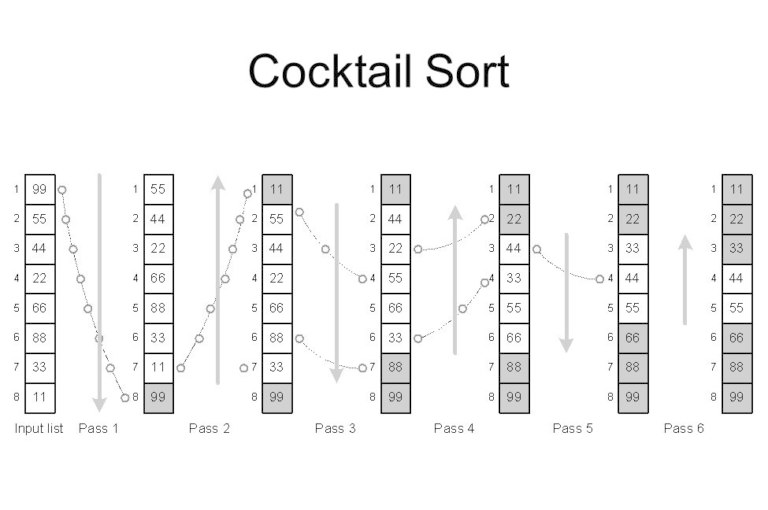
\includegraphics[width=0.75\textwidth]{./imagenes/cocktailsort.png}\\
		Figura 1. CocktailSort\\
	\end{center}
\newpage
		\item GnomeSort.-empieza comparando la primera pareja de valores, si están en orden incrementa el puntero y de nuevo realiza la comparación, si no están en orden, se pasa, el menor a la izquierda y el mayor a la derecha, y se reduce el puntero, ahora la comparación es con el elemento anterior, si no hay un elemento anterior se pasa al siguiente elemento. Cuando el puntero alcanza el extremo superior del array ya está totalmente ordenado.
Cuando compara hacia arriba va sin hacer intercambios, es que el par bajo examen está ordenado entre si, y cuando compara hacia abajo, va haciendo intercambios. El proceso aparece como un zigzagueo continuo a un lado y otro.
La operación empieza por el puntero en el punto más bajo y cuando llega al extremo superior ha terminado de ordenar el array.
		\begin{center}
			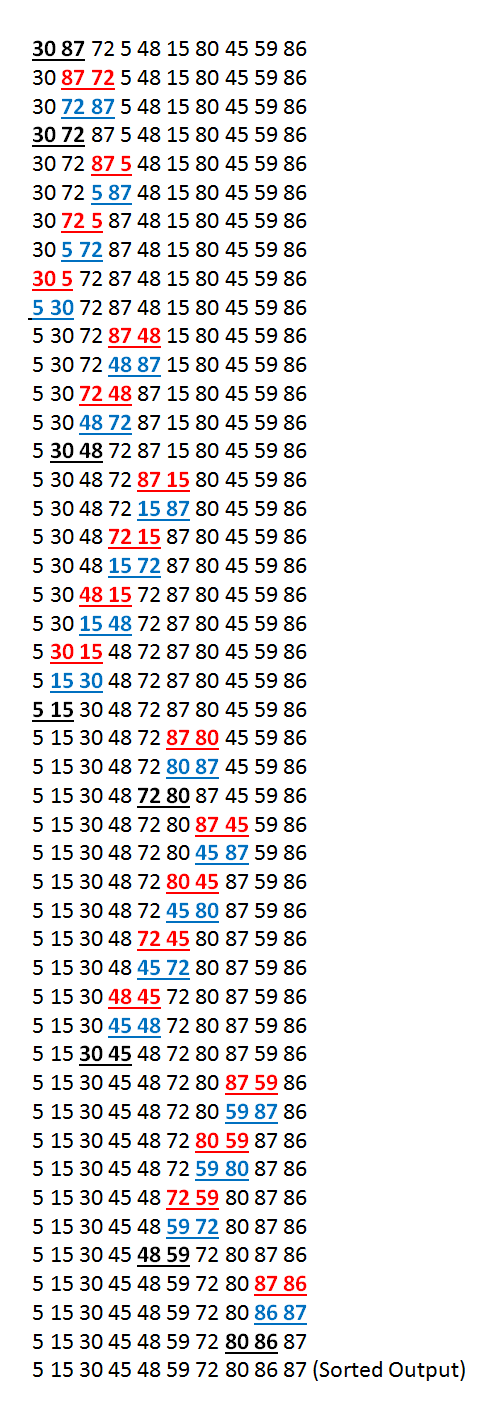
\includegraphics[width=0.30\textwidth]{./imagenes/gnomesort.png}\\
			Figura 2.GnomeSort\\
		\end{center}
\newpage
		\item InsertionSort.- Inicialmente se tiene un solo elemento, que obviamente es un conjunto ordenado. Después, cuando hay k elementos ordenados de menor a mayor, se toma el elemento k+1 y se compara con todos los elementos ya ordenados, deteniéndose cuando se encuentra un elemento menor (todos los elementos mayores han sido desplazados una posición a la derecha) o cuando ya no se encuentran elementos (todos los elementos fueron desplazados y este es el más pequeño). En este punto se inserta el elemento k+1 debiendo desplazarse los demás elementos.
	\begin{center}
		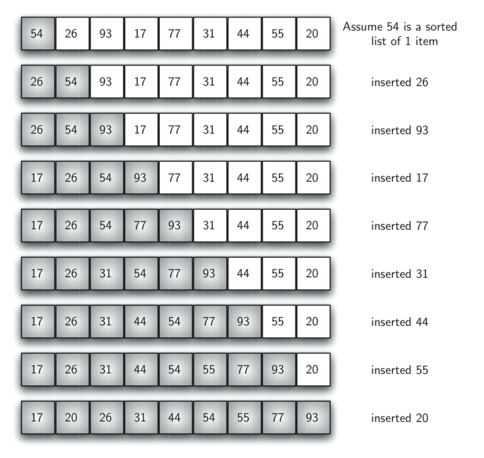
\includegraphics[width=0.55\textwidth]{./imagenes/insertionsort.png}\\
		Figura 3. InsertionSort\\
	\end{center}
	\end{itemize}

	\bigskip
	\newpage
	{\large{\bf ii) Compare el orden de complejidad en el mejor de los casos de manera experimental mediante graficas de sus resultados.}}\\
	
	\bigskip
		\begin{center}
			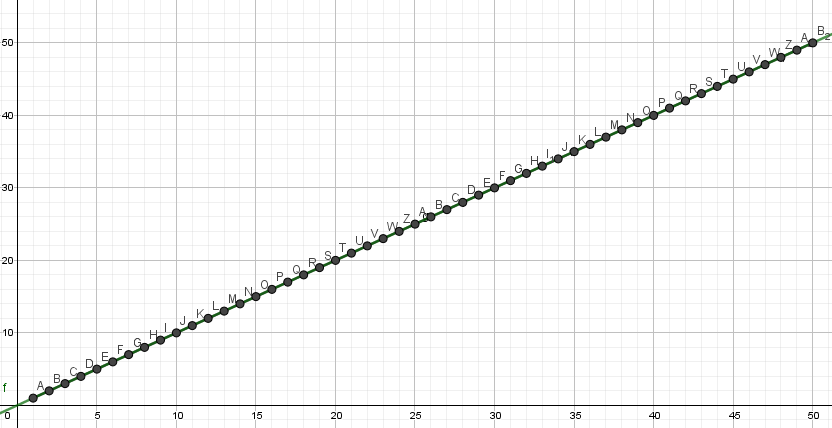
\includegraphics[width=0.55\textwidth]{./imagenes/cocktailMC.PNG}\\
			Figura 4. CocktailSort Mejor de los Casos\\
		\end{center}
	En la figura 4 podemos apreciar la complejidad del algoritmo cuando el se da el mejor de los casos, la cual es lineal, que sería cuando entra el vector ya ordenado, ya que solamente realiza una comprobacion.
		\begin{center}
			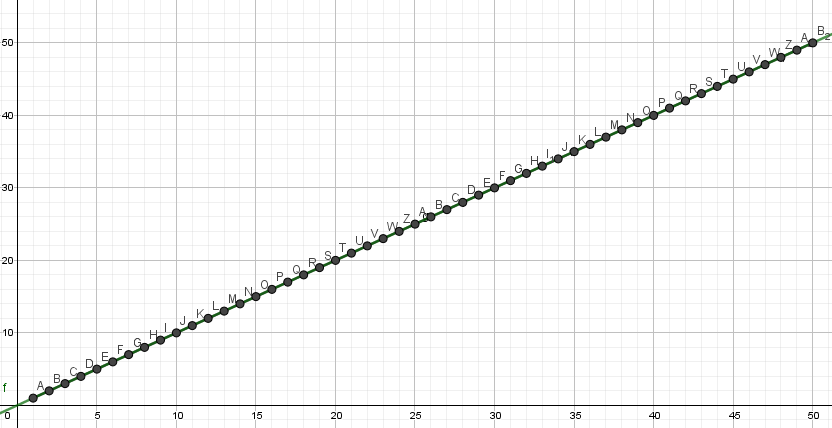
\includegraphics[width=0.55\textwidth]{./imagenes/gnomeMC.PNG}\\
			Figura 5. GnomeSort Mejor de los Casos\\
		\end{center}
En la figura 5 podemos apreciar la complejidad del algoritmo cuando el se da el mejor de los casos, la cual es lineal, que sería cuando entra el vector ya ordenado, ya que solamente realiza una comprobacion.
\newpage
		\begin{center}
			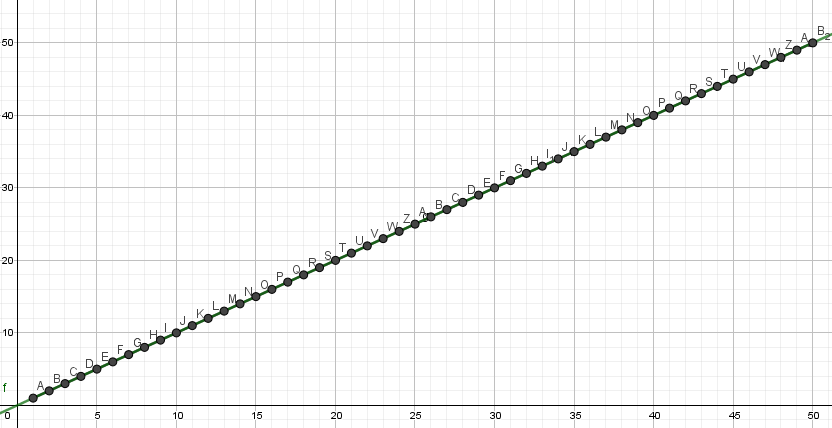
\includegraphics[width=0.55\textwidth]{./imagenes/insertionMC.PNG}\\
			Figura 6. InsertionSort Mejor de los Casos\\
		\end{center}
En la figura 6 podemos apreciar la complejidad del algoritmo cuando el se da el mejor de los casos, la cual es lineal, que sería cuando entra el vector ya ordenado, ya que solamente realiza una comprobacion.
\\\\
Como podemos apreciar, la complejidad de los tres algoritmos es lineal cuando se presenta el mejor de los casos, als er los tres algoritmos basados en el mismo principio, es correcto asumir que su complejidad no varie entre ellos.

\newpage
	{\large{\bf iii) Compare el orden de complejidad en el peor de los casos de manera experimental mediante graficas de sus resultados.}}\\
	
	\bigskip

		\begin{center}
			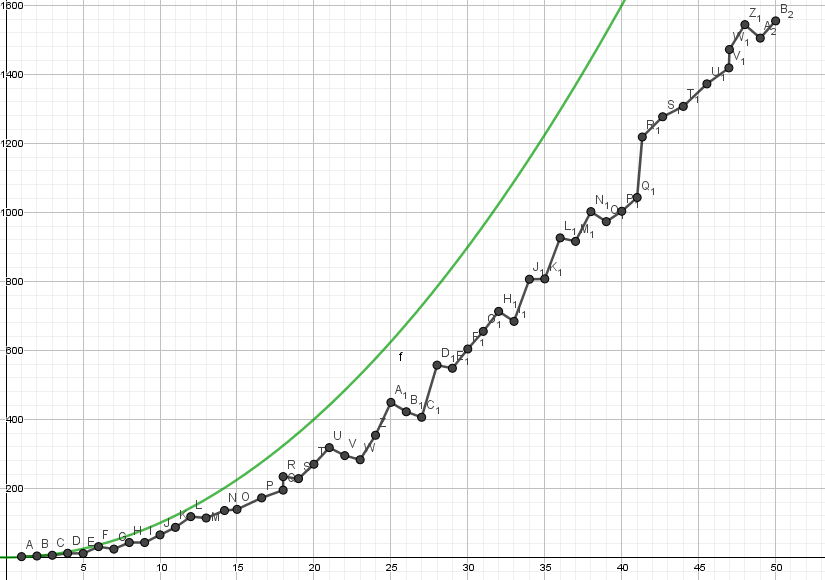
\includegraphics[width=0.55\textwidth]{./imagenes/cocktailPC.png}\\
			Figura 7. CocktailSort Peor de los casos\\
		\end{center}
CocktailSort.- Para este algoritmo, se puede ver un comportamiento creciente, no obstante nunca supera nuestra cota superior propuesta. Por lo tanto, el orden de complejidad de CocktailSort es $$O(n^2)$$.

		\begin{center}
			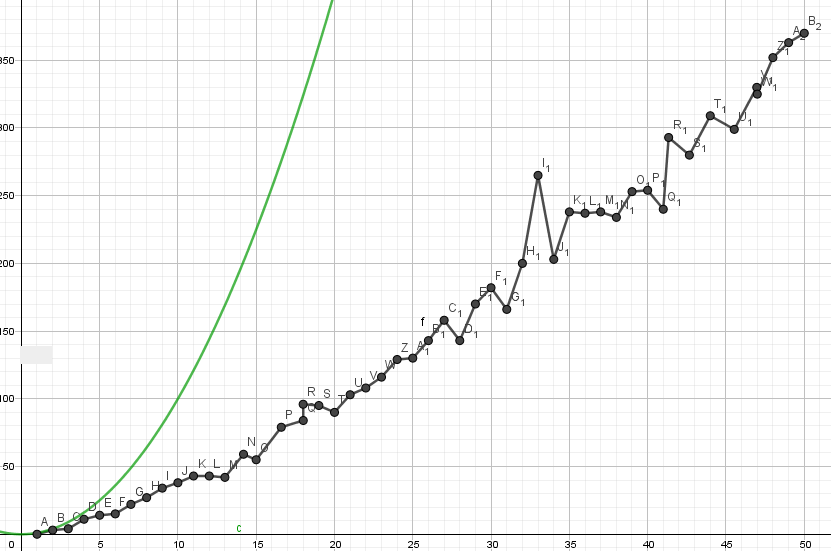
\includegraphics[width=0.55\textwidth]{./imagenes/gnomePC.png}\\
			Figura 8. GnomeSort Peor de los casos\\
		\end{center}
 ShellSort.-Para este algoritmo, se puede ver un comportamiento creciente, no obstante nunca supera nuestra cota superior propuesta. Por lo tanto, el orden de complejidad de ShellSort es $$O(n^2)$$.

		\begin{center}
			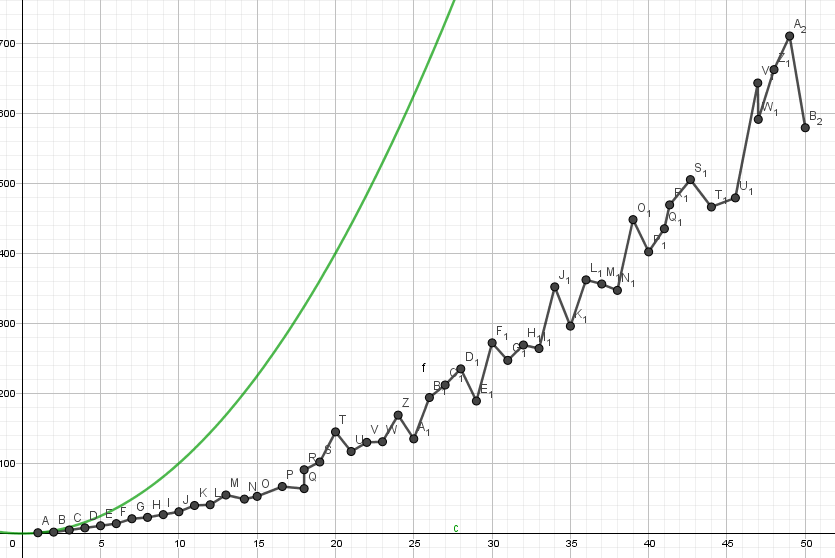
\includegraphics[width=0.55\textwidth]{./imagenes/insertionPC.png}\\
			Figura 9. InsertionSort Peor de los casos\\
		\end{center}
InsertionSot.- Para este algoritmo, se puede ver un comportamiento creciente, no obstante nunca supera nuestra cota 	superior propuesta. Por lo tanto, el orden de complejidad de InsertionSort es $$O(n^2)$$.


	\bigskip

	
	\newpage

	\bigskip

	\section{Conclusi\'on}

	\bigskip

	Volvemos a tocar los algoritmos de ordenacion, estos algoritmos me estan llamando mucho la atencion, me parece muy interesante la manera en la que los pudieron haber pensado y en la forma en la que veian las cosas las personas que los crearon, es algo que no creo que me deje de interesar nunca.\\
Para esta practica volvi a utilizar python debido a su simplicidad a la hora de programar. Tuve algunos problemas para resolver el cocktailSort, pero al final se pudo implementar voliendo a revisar el manual de python.\\
Con esta practica pude darme cuenta que los algoritmos de ordenamiento parten de una base similar y que es por eso que todos tienen una complejidad similar, sin embargo sigo preguntandome como es que sus creadores le hicieron para lograr conseguir que a la hora de lo practico algunos den mejores resultados que otros, es sin duda algo muy interesante e ipnotizante de ver 

	\newpage

	\section{Bibliografía}
	\begin{itemize}
		\item Brassard, G. (1997). Fundamentos de Algoritmia. España: Ed. Prentice Hall. ISBN 848966000X
		\item Harel, D. (2004). Algorithmics: The spirit of Computing (3rd. Ed). Estados Unidos de América: Addison
Wesley. ISBN-13: 978-0321117847
	\end{itemize}


\end{document}